\documentclass{article}

\usepackage[brazil]{babel}
\usepackage[T1]{fontenc}
\usepackage[a4paper, margin=1.5cm]{geometry}
\usepackage[colorlinks, urlcolor=blue, citecolor=red]{hyperref}
\usepackage[utf8]{inputenc}
\usepackage{graphicx}

\title{\textbf{Controlador \emph{fuzzy} para motorista virtual}}
\author{Emmanuel Podestá Jr., Gustavo Zambonin\thanks{
        \texttt{\{emmanuel.podesta,gustavo.zambonin\}@grad.ufsc.br} \hfill
        \texttt{\href{https://github.com/zambonin/ufsc-ine5430}{src/}}
    } \\
    \small{Inteligência Artificial (UFSC -- INE5430)}
}
\date{}

\begin{document}

\maketitle

\section{Introdução}

A lógica difusa (\emph{fuzzy logic}) é uma alternativa muito comum à lógica
Booleana quando mostra-se necessário lidar com o conceito de verdade
não-absoluta, ou parcial; ou seja, quando os valores verdade de variáveis ou
predicados não são exatamente $0$ ou $1$, mas qualquer valor nesta amplitude.
Nestes casos, o valor verdade é geralmente obtido a partir de observações sob
conhecimento inexato ou incompleto, que precisam ser mapeadas de modo a serem
úteis para o raciocínio e a produção de um resultado útil. \medskip

A partir deste modelo, é possível estender o conceito matemático de teoria dos
conjuntos para que estes sejam definidos de modo que seus elementos tenham
níveis de pertinência, generalizando conjuntos clássicos (onde elementos apenas
podem, ou não, pertencer ao conjunto): nota-se que a função de pertinência de
um conjunto clássico retorna apenas valores $0$ ou $1$; em um conjunto difuso,
esta pode gerar valores diferentes. \medskip

Neste trabalho, a lógica difusa é aplicada no contexto de estacionamento de um
``caminhão'', posicionado em um plano cartesiano com certa marcação como o
``alvo''. Esta situação requere várias deduções a partir de conhecimento
não necessariamente correto, na vida real. As ferramentas utilizadas para a
comunicação com o servidor fornecido foram a linguagem Python 3, junto da
biblioteca
\href{https://github.com/scikit-fuzzy/scikit-fuzzy}{\texttt{scikit-fuzzy}},
parte de um ecossistema focado em computação científica e
numérica chamado \href{https://scipy.org}{SciPy}.

\section{Desenvolvimento}

O ``motorista'' recebe a posição atual do caminhão no plano cartesiano, bem
como o ângulo de seu veículo, normalizado a partir de uma simples fórmula,
condizente com o comportamento do servidor. Com estas informações, é
necessário tomar uma decisão sobre como avançar para estacionar da melhor
maneira possível. Utilizando os conjuntos especificados na Figura \ref{fig01},
uma série de regras são aplicadas para determinar o próximo movimento do
caminhão. Tais regras denotam comportamentos de acordo com os dados recebidos.
Alguns exemplos são listados abaixo. É necessário apontar que caso o caminhão
esteja muito próximo de uma das bordas do plano cartesiano, o comportamento do
motorista será indefinido. O caminhão apenas pode movimentar-se ``de ré''.

\begin{itemize}

    \item caso o caminhão esteja no primeiro quadrante e sua parte traseira
        esteja apontando para cima, é necessário virá-lo para a direita, e
        centrá-lo no eixo das abscissas caso necessário;

    \item caso o caminhão esteja no segundo quadrante e sua parte traseira
        esteja virada para a direita, é necessário apenas virá-lo levemente
        para a esquerda até que o ângulo esteja correto, e continuar
        acelerando até o destino;

    \item caso o caminhão esteja no terceiro quadrante, suficientemente perto
        do eixo das abscissas, e sua parte traseira esteja virada para a
        direita, é necessário virá-lo para a direita até que seja possível
        fazer uma nova curva para a esquerda, de modo a centrá-lo neste eixo;

    \item caso o caminhão esteja no quarto quadrante, perto do centro do plano
        cartesiano, com sua parte traseira virada para baixo, o motorista
        deve apenas acelerar e fazer pequenas correções para o lado contrário
        de sua localização no plano;

    \item caso o caminhão esteja no primeiro quadrante e sua parte traseira
        esteja apontando para a esquerda, é necessário virá-lo para a direita
        até que seja possível iniciar uma nova curva para a esquerda, de
        modo a centrá-lo no eixo das abscissas.

\end{itemize}

Vetores numéricos são utilizados para representar o estado do caminhão no
plano cartesiano, compostos de variáveis contendo sua posição, ângulo atual
e o nível de intensidade que uma curva deve ser feita de acordo com estes
dados. Então, uma operação de minimização é aplicada a cada um dos vetores,
construídos de acordo com o comportamento desejado. A minimização funciona,
a grosso modo, de forma análoga a uma porta lógica \texttt{AND}, e serve para
que todas as variáveis numéricas possam influenciar no valor final,
construindo um vetor que representa fielmente a regra. Após este processo, é
necessário maximizar cada uma das coordenadas dos vetores do passo anterior.
A maximização funciona de modo inverso à minimização e representa,
grosseiramente, a aplicação de uma porta \texttt{OR} sobre os vetores, para
que todas as regras sejam consideradas no resultado final. Por fim, ocorre a
``defuzzificação'' destes dados utilizado o método do centroide, escolhido em
virtude do estilo de função de pertinência utilizado -- neste caso,
triangular. \medskip

A escolha dos parâmetros corretos para criar os conjuntos difusos, bem como
a criação de regras para diversos comportamentos que naturalmente seriam
triviais, são pontos que necessitaram de grande atenção no desenvolvimento do
trabalho, visto que ajustes feitos para casos específicos podem vir a afetar
movimentos que seriam óbvios e/ou fáceis de modelar. Assim, buscou-se um
balanço entre a abrangência das regras e o tempo gasto na construção de
``bons'' conjuntos. \medskip

A definição dos intervalos dos conjuntos difusos, por exemplo, precisa de
grande consideração para escolher valores sensatos, de modo a representá-los
corretamente no formato triangular da função de pertinência. Adicionar regiões
nos extremos da amplitude do universo é uma  possível melhoria, que tem como
objetivo melhorar a representação dos dados localizados nos conjuntos. \medskip

O programa responsável por controlar o motorista pode ser encontrado em
\texttt{truck\_driver.py}, e o servidor, em \texttt{fuzzy\_truck\_contest.jar}.
Após executar o JAR e abrir o soquete para comunicação, o ``motorista'' pode
ser iniciado.

\section{Conclusão}

O desenvolvimento do controlador \emph{fuzzy} proporciona aos programadores
grande liberdade para escolha do amálgama de estratégias para produzir um bom
resultado. Embora esta liberdade não seja possível sem seus malefícios (como,
por exemplo, a dificuldade na escolha da combinação de algoritmos, discutida
nos parágrafos anteriores), permite a abrangência de uma maior gama de
problemas. Assim, com a modelagem correta, a lógica difusa faz parte do
ferramental disponíveis em diversos âmbitos, como um modelo matemático que
representa a imprecisão. O ``motorista'' implementado aqui é apenas um simples
exemplo, utilizado de modo didático para introduzir tais conceitos.

\begin{figure}[ht]
    \centering
    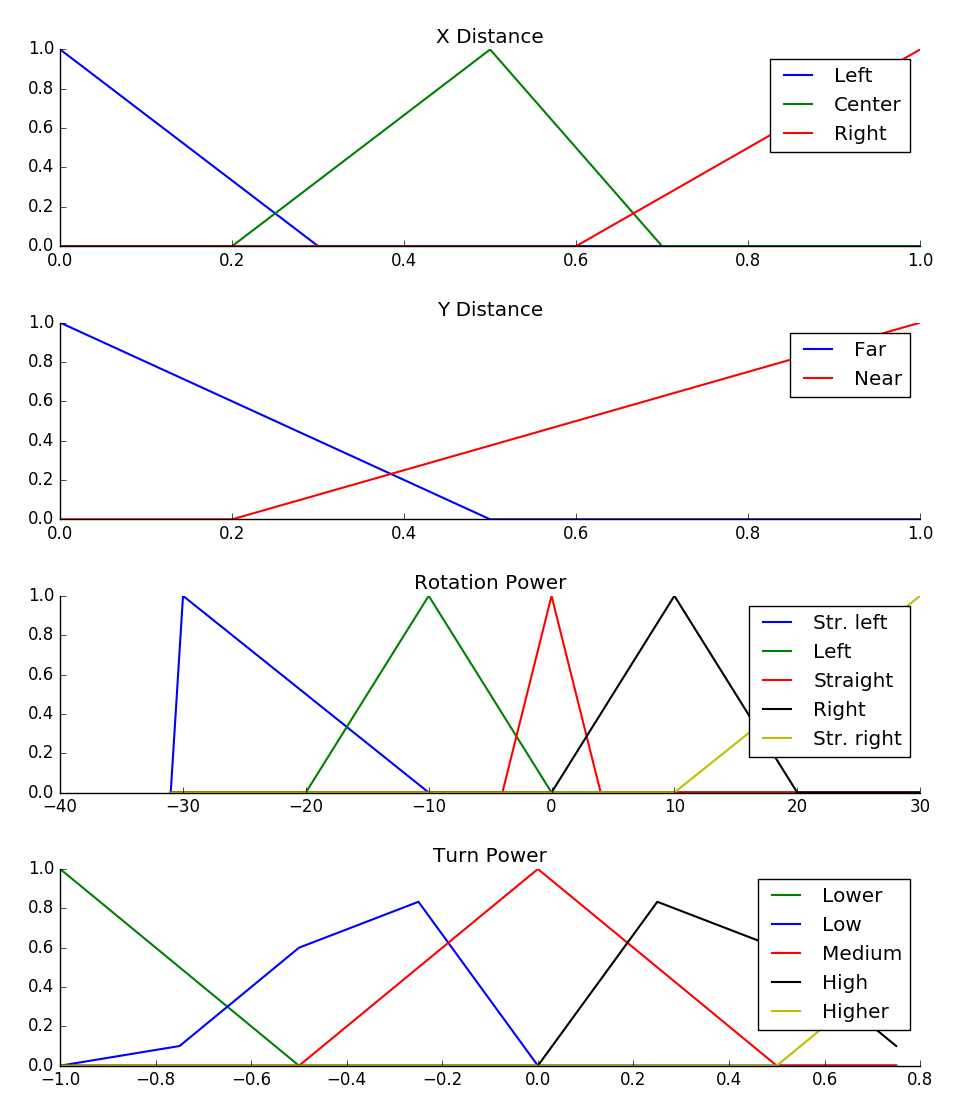
\includegraphics[scale=0.45]{figure_1}
    \caption{Conjuntos utilizados na definição do problema. Respectivamente,
        mostram a posição do caminhão no eixo das abscissas e das ordenadas
        (em um intervalo $[0, 1]$), ângulo em que o caminhão se encontra (em
        um intervalo normalizado $[0, 360] \longrightarrow [-30, 30]$) e
        quanto este deve virar (por limitações do servidor, o veículo deve
        girar no máximo 30º para um dos lados, e isto é fornecido ao servidor
        como um valor dentro do intervalo $[-1, 1]$). Não foi necessário a
        definição de uma terceira partição para classificar a posição do
        caminhão no eixo das ordenadas.}
    \label{fig01}
\end{figure}

\end{document}
